\documentclass[12pt]{article}
\usepackage{longtable}
\usepackage{titling}
\usepackage{setspace}
\usepackage{hyperref}
\usepackage{lipsum}
\usepackage{graphicx}
\usepackage[margin=1in]{geometry}

\newcommand{\PutTitle}[1]
{ \begin{center}
        {\huge\bfseries\thetitle}\\
        by \theauthor\\
        \thedate\\
        #1        
    \end{center}
    \hrule
    \vspace{2ex}
}

\setlength\paperwidth{8.5in}
\setlength\paperheight{11in}
\setlength\parindent{24pt}

\hypersetup
{
    colorlinks=true,
    linkcolor=blue,
    urlcolor=blue,
}

\begin{document}

\title{Tumble Buggy}
\author{Jonah Mondragon}
\date{\today}
\PutTitle{Physics Period 6}

\doublespacing

The purpose is to devise an experiment that will demonstrate the principals of
constant speed.

\begin{figure}[h]
    \centering
    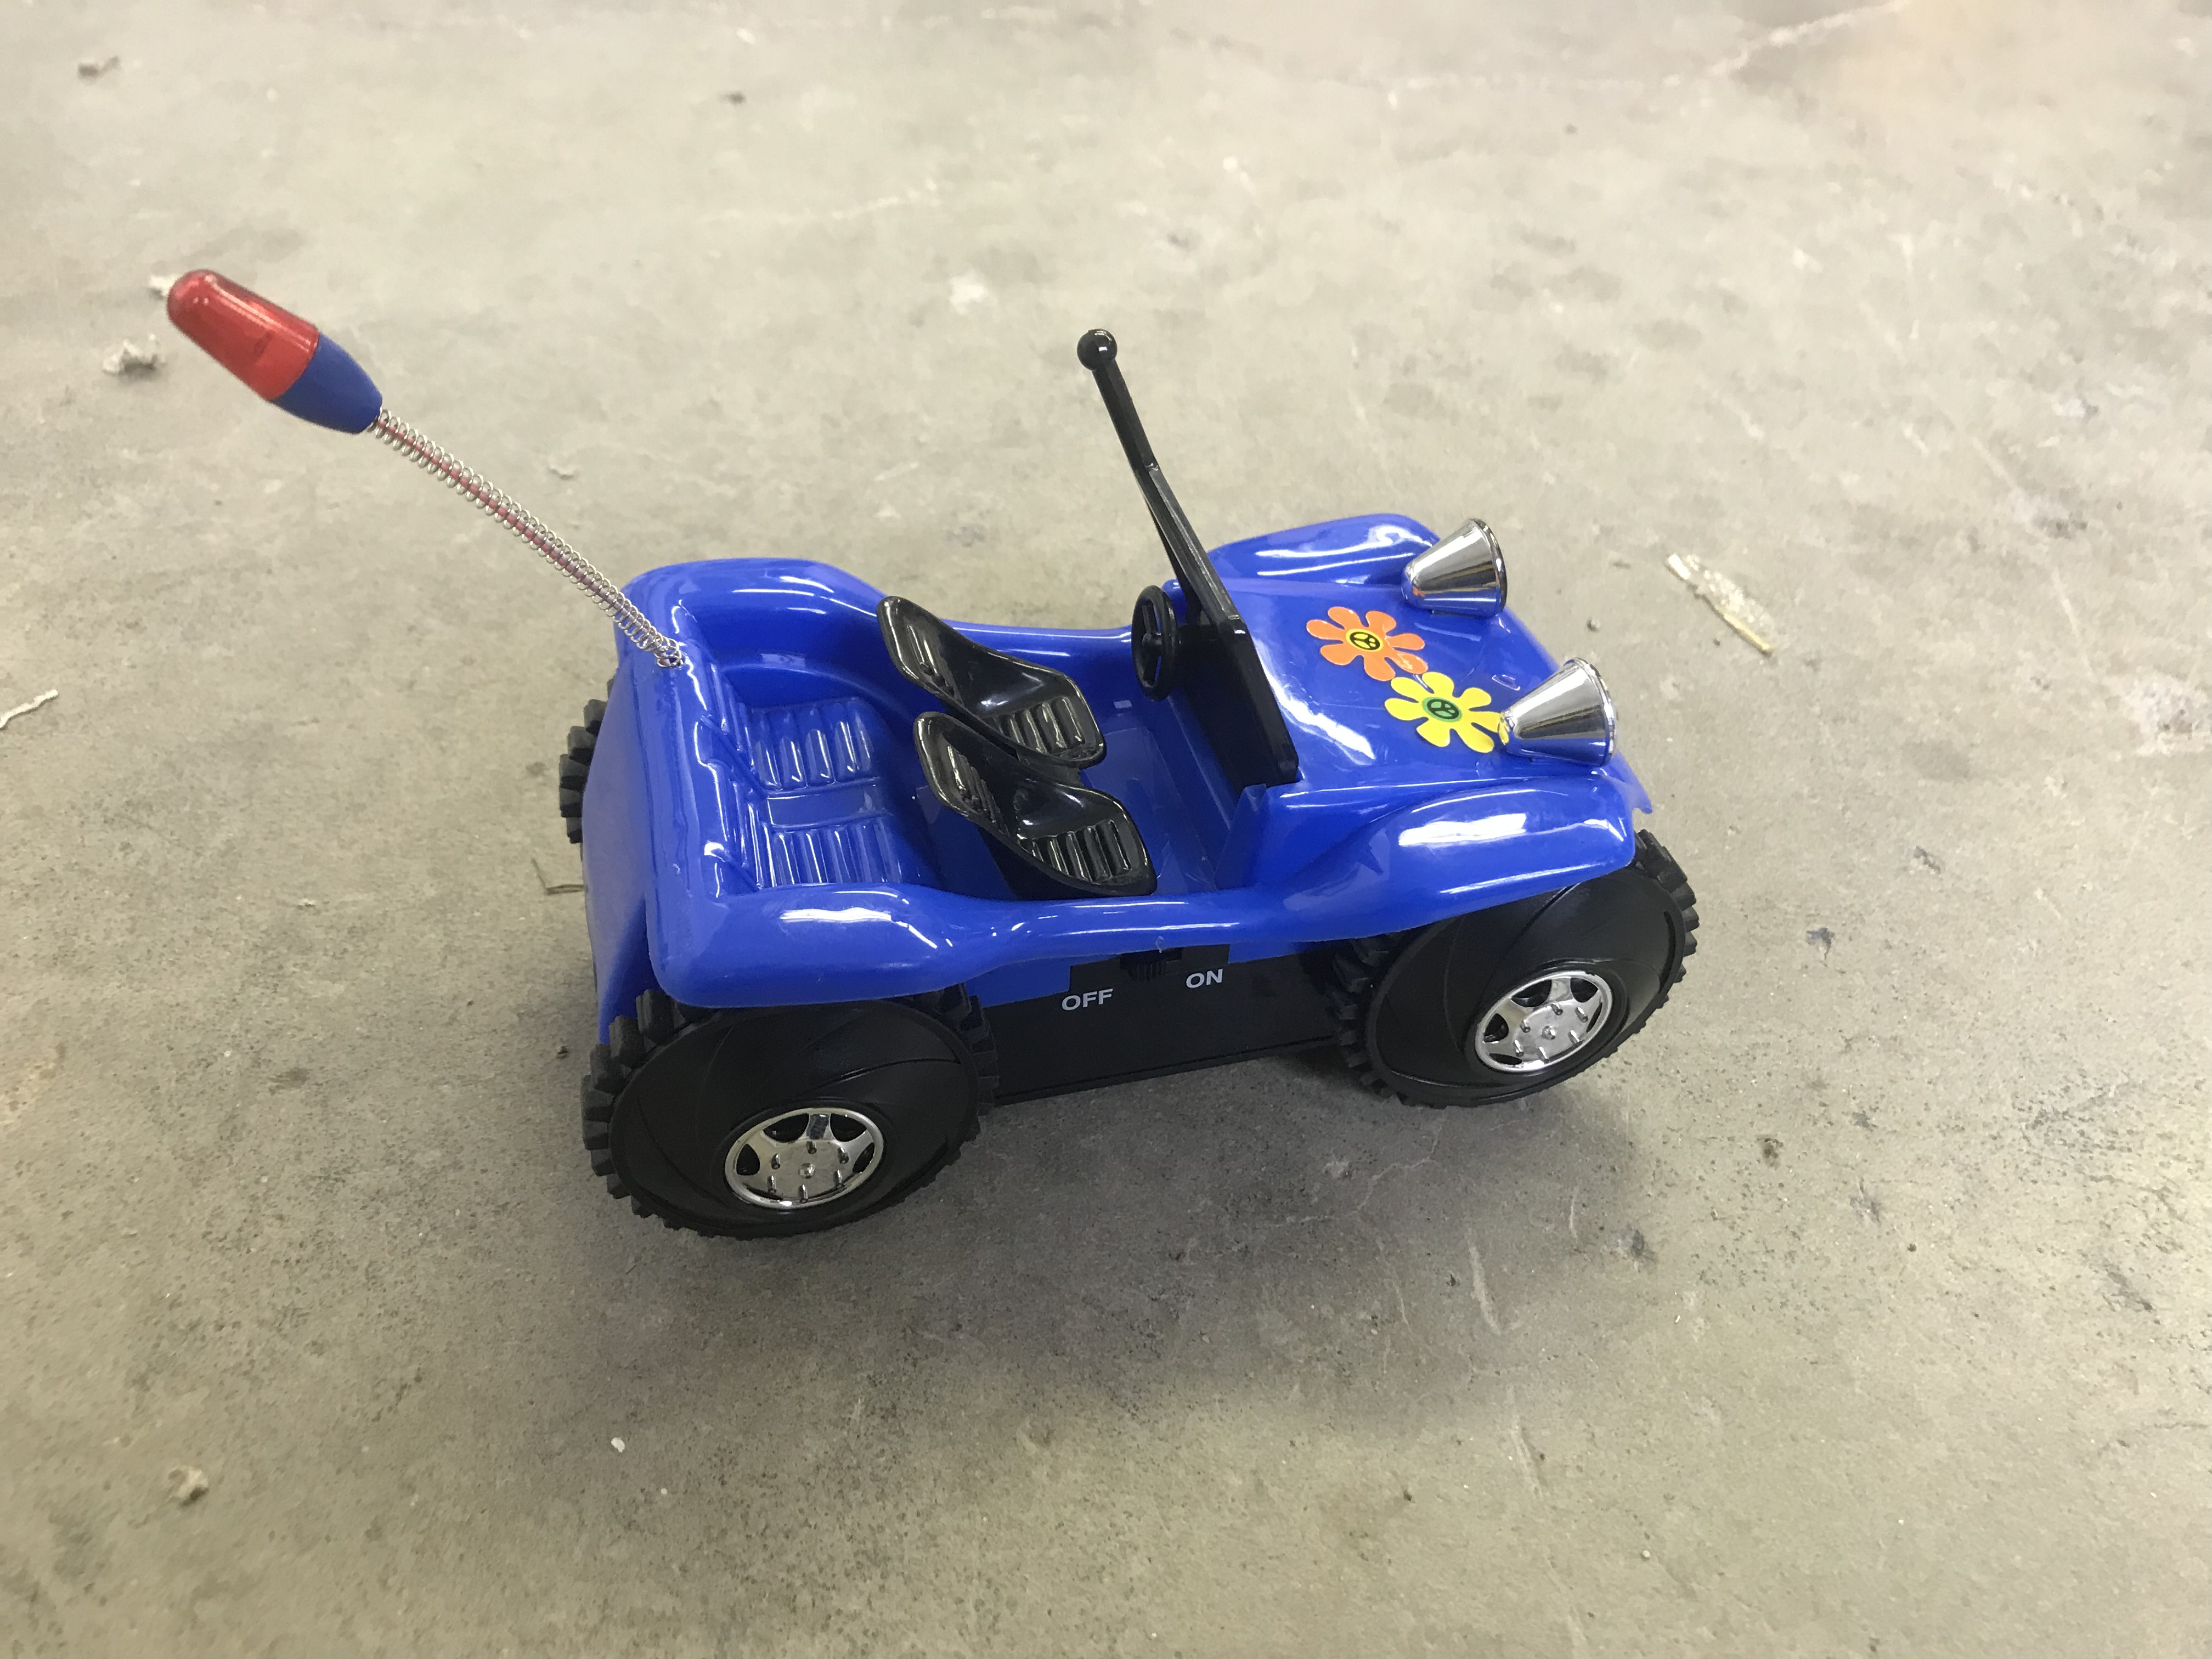
\includegraphics[width=4.25in]{tumble_buggy.jpg}
    \caption{Tumble Buggy}
    \label{figure:buggy}
\end{figure}

The methodology for this experiment will involve measuring the speed of the
above toy tumble buggy (Figure \ref{figure:buggy}). Simply measuring the time it
takes to travel a distance won't accomplish this endeavor as it won't
incorporate position further than that determined by the chosen distance;
therefore I've elected to measure the linear distance from a starting point to
points determined by an interval of two seconds. The latter approach
incorporates position and compares it to time; and linearly measuring the growth
in distance from the starting point at every interval will accommodate the
slight curve this tumble buggy tends to drive in. The intervals will be marked
with sandbags, they'll be dropped at the position the tumble buggy is in at the
end of every interval, after five intervals, the distance will be measured from
the starting point to each sandbag and then input into the data into a table
(table \ref{table:data}), the process will be repeated two more times and then
the data graphed with Excel (figure \ref{figure:data}).

\begin{table}
    \centering
    Tumble Buggy Position (meters) vs. Time\\
    \begin{tabular}{|l|l|l|l|}
    \hline
        Period (seconds) & Trial 1 & Trial 2 & Trial 3 \\ \hline
        2 & 0.71 & 0.757 & 0.64 \\ \hline
        4 & 1.27 & 1.25 & 1.01 \\ \hline
        6 & 1.85 & 1.62 & 1.54 \\ \hline
        8 & 2.35 & 2.17 & 1.98 \\ \hline
        10 & 2.83 & 2.67 & 2.35 \\ \hline
    \end{tabular}
    \caption{Raw data from experiment}
    \label{table:data}
\end{table}

\begin{figure}
    \centering
    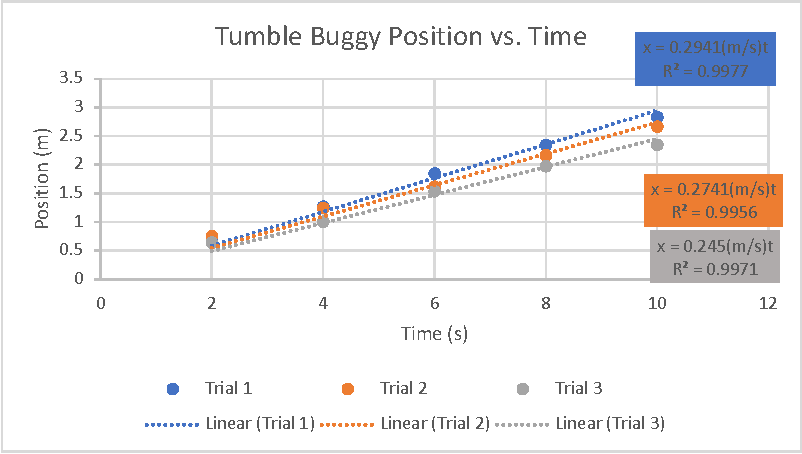
\includegraphics{tumble_buggy_position_vs_time_graph.pdf}
    \caption{Graph representation of the data in table \ref{table:data}}
    \label{figure:data}
\end{figure}

As we can see from the data (table \ref{table:data} and figure
\ref{figure:data}), the tumble buggy moves at a constant speed of, taking the
average from the three trials,
27.11 centimeters per second. We see from the equations in figure
\ref{figure:data} that we have accurate results as the $R^2$ value is extremely
close to $1$ for all three trials.

\end{document}

